% Template for PLoS
% Version 3.6 Aug 2022
%
% % % % % % % % % % % % % % % % % % % % % %
%
% -- IMPORTANT NOTE
%
% This template contains comments intended
% to minimize problems and delays during our production
% process. Please follow the template instructions
% whenever possible.
%
% % % % % % % % % % % % % % % % % % % % % % %
%
% Once your paper is accepted for publication,
% PLEASE REMOVE ALL TRACKED CHANGES in this file
% and leave only the final text of your manuscript.
% PLOS recommends the use of latexdiff to track changes during review, as this will help to maintain a clean tex file.
% Visit https://www.ctan.org/pkg/latexdiff?lang=en for info or contact us at latex@plos.org.
%
%
% There are no restrictions on package use within the LaTeX files except that no packages listed in the template may be deleted.
%
% Please do not include colors or graphics in the text.
%
% The manuscript LaTeX source should be contained within a single file (do not use \input, \externaldocument, or similar commands).
%
% % % % % % % % % % % % % % % % % % % % % % %
%
% -- FIGURES AND TABLES
%
% Please include tables/figure captions directly after the paragraph where they are first cited in the text.
%
% DO NOT INCLUDE GRAPHICS IN YOUR MANUSCRIPT
% - Figures should be uploaded separately from your manuscript file.
% - Figures generated using LaTeX should be extracted and removed from the PDF before submission.
% - Figures containing multiple panels/subfigures must be combined into one image file before submission.
% For figure citations, please use "Fig" instead of "Figure".
% See http://journals.plos.org/plosone/s/figures for PLOS figure guidelines.
%
% Tables should be cell-based and may not contain:
% - spacing/line breaks within cells to alter layout or alignment
% - do not nest tabular environments (no tabular environments within tabular environments)
% - no graphics or colored text (cell background color/shading OK)
% See http://journals.plos.org/plosone/s/tables for table guidelines.
%
% For tables that exceed the width of the text column, use the adjustwidth environment as illustrated in the example table in text below.
%
% % % % % % % % % % % % % % % % % % % % % % % %
%
% -- EQUATIONS, MATH SYMBOLS, SUBSCRIPTS, AND SUPERSCRIPTS
%
% IMPORTANT
% Below are a few tips to help format your equations and other special characters according to our specifications. For more tips to help reduce the possibility of formatting errors during conversion, please see our LaTeX guidelines at http://journals.plos.org/plosone/s/latex
%
% For inline equations, please be sure to include all portions of an equation in the math environment.  For example, x$^2$ is incorrect; this should be formatted as $x^2$ (or $\mathrm{x}^2$ if the romanized font is desired).
%
% Do not include text that is not math in the math environment. For example, CO2 should be written as CO\textsubscript{2} instead of CO$_2$.
%
% Please add line breaks to long display equations when possible in order to fit size of the column.
%
% For inline equations, please do not include punctuation (commas, etc) within the math environment unless this is part of the equation.
%
% When adding superscript or subscripts outside of brackets/braces, please group using {}.  For example, change "[U(D,E,\gamma)]^2" to "{[U(D,E,\gamma)]}^2".
%
% Do not use \cal for caligraphic font.  Instead, use \mathcal{}
%
% % % % % % % % % % % % % % % % % % % % % % % %
%
% Please contact latex@plos.org with any questions.
%
% % % % % % % % % % % % % % % % % % % % % % % %

\documentclass[10pt,letterpaper]{article}
\usepackage[top=0.85in,left=2.75in,footskip=0.75in]{geometry}

% amsmath and amssymb packages, useful for mathematical formulas and symbols
\usepackage{amsmath,amssymb}

% Use adjustwidth environment to exceed column width (see example table in text)
\usepackage{changepage}

% textcomp package and marvosym package for additional characters
\usepackage{textcomp,marvosym}

% cite package, to clean up citations in the main text. Do not remove.
\usepackage{cite}

% Use nameref to cite supporting information files (see Supporting Information section for more info)
\usepackage{nameref,hyperref}

% line numbers
\usepackage[right]{lineno}

% ligatures disabled
\usepackage[nopatch=eqnum]{microtype}
\DisableLigatures[f]{encoding = *, family = * }

% color can be used to apply background shading to table cells only
\usepackage[table]{xcolor}

% array package and thick rules for tables
\usepackage{array}

% create "+" rule type for thick vertical lines
\newcolumntype{+}{!{\vrule width 2pt}}

% create \thickcline for thick horizontal lines of variable length
\newlength\savedwidth
\newcommand\thickcline[1]{%
  \noalign{\global\savedwidth\arrayrulewidth\global\arrayrulewidth 2pt}%
  \cline{#1}%
  \noalign{\vskip\arrayrulewidth}%
  \noalign{\global\arrayrulewidth\savedwidth}%
}

% \thickhline command for thick horizontal lines that span the table
\newcommand\thickhline{\noalign{\global\savedwidth\arrayrulewidth\global\arrayrulewidth 2pt}%
\hline
\noalign{\global\arrayrulewidth\savedwidth}}

% Remove comment for double spacing
%\usepackage{setspace}
%\doublespacing

% Text layout
\raggedright
\setlength{\parindent}{0.5cm}
\textwidth 5.25in
\textheight 8.75in

% Bold the 'Figure #' in the caption and separate it from the title/caption with a period
% Captions will be left justified
\usepackage[aboveskip=1pt,labelfont=bf,labelsep=period,justification=raggedright,singlelinecheck=off]{caption}
\renewcommand{\figurename}{Fig}

% Use the PLoS provided BiBTeX style
\bibliographystyle{plos2015}

% Remove brackets from numbering in List of References
\makeatletter
\renewcommand{\@biblabel}[1]{\quad#1.}
\makeatother

% Header and Footer with logo
\usepackage{lastpage,fancyhdr,graphicx}
\usepackage{epstopdf}
%\pagestyle{myheadings}
\pagestyle{fancy}
\fancyhf{}
%\setlength{\headheight}{27.023pt}
%\lhead{\includegraphics[width=2.0in]{PLOS-submission.eps}}
\rfoot{\thepage/\pageref{LastPage}}
\renewcommand{\headrulewidth}{0pt}
\renewcommand{\footrule}{\hrule height 2pt \vspace{2mm}}
\fancyheadoffset[L]{2.25in}
\fancyfootoffset[L]{2.25in}
\lfoot{\today}

%% Include all macros below

\newcommand{\lorem}{{\bf LOREM}}
\newcommand{\ipsum}{{\bf IPSUM}}

%% END MACROS SECTION


%% MY PACKAGE
\usepackage[detect-all=true]{siunitx}
\sisetup{
    round-mode = places,
    round-precision = 2
}

\usepackage{pifont}% http://ctan.org/pkg/pifont
\newcommand{\cmark}{\ding{51}}%
\newcommand{\xmark}{\ding{55}}%

\usepackage{booktabs}
\usepackage{minted}
\usepackage[acronym, style=index, shortcuts]{glossaries-extra}
\setabbreviationstyle[acronym]{long-short}

% define new commands
%\makeglossaries
\newacronym{blat}{BLAT}{BLAST-like alignment tool}
\newacronym{blast}{BLAST}{Basic Local Alignment Search Tool}
\newacronym{cli}{CLI}{Command-Line Interface}
\newacronym{api}{API}{Application Programming Interface}
\newacronym{ide}{IDE}{Integrated Development Environment}
\newacronym{gil}{GIL}{Global Interpreter Lock}
\newacronym{ci}{CI}{Continuous Integration}
\newacronym{cd}{CD}{Continuous Development}
\newacronym{ucsc}{UCSC}{UCSC Genome Browser}
\newacronym{hsp}{HSP}{High-Scoring Pair}
\newglossaryentry{pxblat}{name=PxBLAT, description={pxblat}}
%% MY PACKAGE

\begin{document}
\vspace*{0.2in}

% Title must be 250 characters or less.
\begin{flushleft}
	{\Large
		\textbf\newline{PxBLAT: An efficient python binding library for BLAT} % Please use "sentence case" for title and headings (capitalize only the first word in a title (or heading), the first word in a subtitle (or subheading), and any proper nouns).
	}
	\newline
	% Insert author names, affiliations and corresponding author email (do not include titles, positions, or degrees).
	\\
	Yangyang Li\textsuperscript{1},
	%	Name2 Surname\textsuperscript{2\Yinyang},
	%	Name3 Surname\textsuperscript{2,3\textcurrency},
	%	Name4 Surname\textsuperscript{2},
	%	Name5 Surname\textsuperscript{2\ddag},
	%	Name6 Surname\textsuperscript{2\ddag},
	Rendong Yang\textsuperscript{1*}
	%	with the Lorem Ipsum Consortium\textsuperscript{\textpilcrow}
	\\
	\bigskip
	\textbf{1} Department of Urology, Northwestern University Feinberg School of Medicine, Chicago, IL, USA
	%	\\
	%	\textbf{2} Affiliation Dept/Program/Center, Institution Name, City, State, Country
	%	\\
	%	\textbf{3} Affiliation Dept/Program/Center, Institution Name, City, State, Country
	%	\\
	\bigskip

	% Insert additional author notes using the symbols described below. Insert symbol callouts after author names as necessary.
	%
	% Remove or comment out the author notes below if they aren't used.
	%
	% Primary Equal Contribution Note
	%	\Yinyang These authors contributed equally to this work.

	% Additional Equal Contribution Note
	% Also use this double-dagger symbol for special authorship notes, such as senior authorship.
	%	\ddag These authors also contributed equally to this work.

	% Current address notes
	%	\textcurrency Current Address: Dept/Program/Center, Institution Name, City, State, Country % change symbol to "\textcurrency a" if more than one current address note
	% \textcurrency b Insert second current address
	% \textcurrency c Insert third current address

	% Deceased author note
	%	\dag Deceased

	% Group/Consortium Author Note
	%	\textpilcrow Membership list can be found in the Acknowledgments section.

	% Use the asterisk to denote corresponding authorship and provide email address in note below.
	* rendong.yang@northwestern.edu

\end{flushleft}
% Please keep the abstract below 300 words
\section*{Abstract}
\gls{pxblat}, a Python library, is introduced to address the limitations inherent in the traditional \gls{blat} suite, offering significant improvements in terms of usability, performance, and integration within the Python ecosystem. In our manuscript, we present a detailed comparison of \gls{pxblat} against BLAT, demonstrating notable advancements in execution speed, data handling, and user interaction capabilities. Benchmarked across multiple datasets, \gls{pxblat} shows a considerable speedup ranging from 1.00 to 1.77 times, underscoring its efficiency and potential to streamline genomic data analysis workflows. Furthermore, we highlight the accessibility of \gls{pxblat}, including its code and comprehensive documentation, all aimed at fostering community engagement and facilitating easy adoption.


%
%\gls{pxblat}, a Python library, is designed to enhance usability and efficiency in interacting with the \gls{blat}.
%\gls{pxblat} provides an intuitive \gls{api} design, allowing the incorporation of its functionality directly into Python-based bioinformatics workflows.
%Moreover, \gls{pxblat}'s design philosophy emphasizes ease of use, memory efficiency, and the elimination of intermediary files and unnecessary system calls, thereby enhancing computational speed and user experience.
%Benchmark tests reveal its superior performance across various datasets, illustrating its capacity to maintain correctness.
%\gls{pxblat} supports Python (version 3.9+), and pre-compiled packages are released via PyPI (\url{https://pypi.org/project/pxblat/}) and Bioconda (\url{https://anaconda.org/bioconda/pxblat}).
%The source code and executable are freely available for academic, nonprofit, and personal use.
%Commercial licensing information is available on the Kent Informatics website (\url{http://www.kentinformatics.com}).
%Its documentation is available on ReadTheDocs (\url{https://pxblat.readthedocs.io/en/latest/}).
%\textbf{Availability and Implementation:}

% Please keep the Author Summary between 150 and 200 words
% Use first person. PLOS ONE authors please skip this step.
% Author Summary not valid for PLOS ONE submissions.
%\section*{Author summary}
%Lorem ipsum dolor sit amet, consectetur adipiscing elit. Curabitur eget porta erat. Morbi consectetur est vel gravida pretium. Suspendisse ut dui eu ante cursus gravida non sed sem. Nullam sapien tellus, commodo id velit id, eleifend volutpat quam. Phasellus mauris velit, dapibus finibus elementum vel, pulvinar non tellus. Nunc pellentesque pretium diam, quis maximus dolor faucibus id. Nunc convallis sodales ante, ut ullamcorper est egestas vitae. Name sit amet enim ultrices, ultrices elit pulvinar, volutpat risus.

\linenumbers

% Use "Eq" instead of "Equation" for equation citations.
\section*{Introduction}
The rise of Python as a preferred programming language within bioinformatics is widely acknowledged as a result of its user-friendly nature, extensive libraries, and unparalleled versatility~\cite{perkel2015programming}.
A variety of libraries have been crafted to augment Python's interface, thereby amplifying the adaptability and compatibility of bioinformatics tools~\cite{putri2022analysing, cock2009biopython}.
For instance, Biopython~\cite{cock2009biopython}, a preeminent bioinformatics library, furnishes interfaces to tools like \gls{blast}~\cite{altschul1990basic} and Clustal~\cite{higgins1988clustal}.
\gls{blat}, a prominent tool in bioinformatics, is renowned for its speed in genome sequence alignments and serves as a more efficient alternative to \gls{blast} for aligning DNA sequences with the reference genome~\cite{kent2002blat}.
Furthermore, the unprecedented growth in genome sequencing technologies has significantly increased the availability of genomic data, emphasizing the need for advanced tools in both research and clinical contexts~\cite{mardis2008next,marx2023method}.

However, despite its popularity and effectiveness, \gls{blat}'s integration is fraught with difficulties, primarily due to its C-based implementation and reliance on \glspl{cli}, hindering seamless integration into Python projects.
Also, executing extensive queries with the \gls{blat} suite leads to inefficiencies, particularly when operations are isolated and not executed in batches.
Typically, \gls{blat}'s task allocation is sporadic, intermixed with other tasks.
Users generally face a choice: either employ standalone \gls{blat} or integrate \emph{gfServer} with \emph{gfClient}~\cite{altschul1990basic}.
\gls{blat}'s standard operational model involves initiating \emph{gfServer}, conducting the sequence query through \emph{gfClient}, and subsequently terminating the server after each query.
This method becomes highly inefficient for ungrouped, numerous queries as it necessitates the repeated initialization and shutdown of \emph{gfServer}, introducing significant overhead~\cite{kent2002blat}.
An optimized approach would entail initiating \emph{gfServer} a single time and leveraging \emph{gfClient} to execute multiple queries.
However, the command-line-only access to \emph{gfServer} and \emph{gfClient} complicates this process.
This limitation necessitates the management of system calls (like \emph{subprocess} or \emph{os.system}), the handling of intermediate temporary files, and dealing with format conversion, all of which cumulatively degrade performance.

\gls{pxblat} is proposed as a solution that allows for the programmatic use of \gls{blat}, ensuring its smooth integration into new algorithms or analytical pipelines within the Python ecosystem.
It acts as a conduit, merging the high-performance capabilities of \gls{blat} with Python's versatility while ensuring data reproducibility.
The primary goal of \gls{pxblat} is to bridge the gap in the current landscape by providing a Python binding library tailored specifically for \gls{blat}, addressing both the efficiency bottlenecks and the ergonomic challenges of its integration.

\section*{Design and implementation}
%\subsection*{Etiam eget sapien nibh}
% For figure citations, please use "Fig" instead of "Figure".
% Place figure captions after the first paragraph in which they are cited.
%\begin{figure}[!h]
%	\caption{{\bf Bold the figure title.}
%		Figure caption text here, please use this space for the figure panel descriptions instead of using subfigure commands. A: Lorem ipsum dolor sit amet. B: Consectetur adipiscing elit.}
%	\label{fig1}
%\end{figure}
The design of \gls{pxblat} is anchored in the principles of readability and simplicity, fostering an intuitive user interface that minimizes the learning curve for users.
In our quest to streamline complexity and amplify both usability and performance, we meticulously extracted the core implementation of \gls{blat} from the broader \gls{ucsc} codebase, significantly reducing dependency overhead.

We preserved the integrity of the original C codebase while reimplementing key \gls{blat} \(\left(\mathtt{V}37.1\right)\) utilities such as \emph{faTwoBit}, \emph{gfServer}, and \emph{gfClient} in C\texttt{++}.
This strategic choice not only modernizes the code but also enhances maintainability and scalability.
The integration of the revamped C\texttt{++} code with \gls{pxblat} was achieved using Pybind11~\cite{pybind11}, a lightweight, seamless method for interfacing C\texttt{++} and Python.

This approach ensures a direct and efficient interaction with \gls{blat}'s functions, upholding the original performance benchmarks and reliability of \gls{blat}.
Simultaneously, it extends the framework's functionality, aligning it with modern computational standards and making it a robust tool in the bioinformatics toolkit (Table~\ref{tab:apicmp}).

\begin{table}[!ht]
	\centering
	\caption{{\bf Overview of features of \gls{pxblat} compared with \gls{blat}.}}\label{tab:apicmp}
	\begin{tabular}{@{}lll@{}}
		\toprule
		Feature          & \gls{pxblat} & \gls{blat} \\ \midrule
		start server     & \cmark{}     & \cmark{}   \\
		stop  server     & \cmark{}     & \cmark{}   \\
		query server     & \cmark{}     & \cmark{}   \\
		wait server      & \cmark{}     & \xmark{}   \\
		fasta to bit     & \cmark{}     & \xmark{}   \\
		bit to fasta     & \cmark{}     & \xmark{}   \\
		port retry       & \cmark{}     & \xmark{}   \\
		shell completion & \cmark{}     & \xmark{}   \\
		\bottomrule
	\end{tabular}
	\begin{flushleft}
		This table presents a comprehensive comparison between the features offered by \gls{pxblat} and \gls{blat}.
		Features are denoted with a \cmark{} to signify availability and an \xmark{} to indicate absence.
		Notably, \gls{pxblat} showcases significant enhancements, particularly in server management (e.g., wait server), data conversion (e.g., fasta to bit, bit to fasta), and enriched user interaction (e.g., shell completion).
		These advancements firmly establish \gls{pxblat} as a superior and more versatile alternative to the conventional \gls{blat} tool.
	\end{flushleft}
\end{table}

\gls{pxblat} delivers its query results in alignment with the \emph{QueryResult} class of Biopython~\cite{cock2009biopython}, enabling seamless manipulation of query outputs (Listing~\ref{listing:example}).
This integration effectively streamlines the post-query workflow, allowing users to leverage the full potential of Biopython in their sequence alignment tasks.
Significantly, \gls{pxblat} negates the necessity for intermediate files by conducting all operations in memory.
This advancement eliminates the often cumbersome and time-consuming step of data format conversion, enabling users to concentrate on the core aspects of sequence alignment.
To enhance user flexibility, the necessity for input and output files has been made optional, aligning with diverse user preferences and workflows.

\begin{listing}
	\inputminted[breaklines]{python}{code/example1.py}
	\caption{{\bf \gls{api} Example.} The code snippet shows how to use the \gls{api} of \gls{pxblat},
		and the query result can be iterated. More code examples can be found at \url{https://pxblat.readthedocs.io/en}}
	\label{listing:example}
\end{listing}

Recognizing the latency and potential performance bottlenecks induced by system calls, \gls{pxblat} minimizes their usage, thereby streamlining operations and enhancing overall efficiency.
Additionally, \gls{pxblat} simplifies server status retrieval, circumventing the complexities and potential pitfalls of log file manipulation, particularly in concurrent usage scenarios.
To further elevate the user experience and operational efficiency, \gls{pxblat} integrates several ergonomic features.
These include real-time server readiness checks for alignments, automatic port retries when the default is in use, and the capability to latch onto an already running server if available.
These features collectively ensure a smoother, more efficient alignment process, reducing downtime and maximizing productivity.

To facilitate a smooth user onboarding experience, we offer an extensive range of examples and comprehensive documentation (Listing~\ref{listing:example}).
\gls{pxblat} introduces a robust set of \glspl{api}, including the classes \emph{Server} and \emph{Client}, along with a suite of functions designed to replicate the capabilities of the \gls{blat} suite.
These classes mirror the utilities of the \gls{cli} tools \emph{gfServer} and \emph{gfClient}, respectively, but with added flexibility to accommodate a wider range of user requirements.
Key functions such as \emph{start\_server}, \emph{query\_server}, \emph{status\_server}, \emph{fa2twobit}, and \emph{twobit2fa} are provided to cater to diverse usage scenarios.
Rigorous testing and development protocols, incorporating \gls{ci} and \gls{cd}, have been employed to ensure high code quality and reliability.

Moreover, \gls{pxblat} utilizes type annotations in its public classes and functions.
This not only reinforces code quality and correctness through type checking and static analysis but also enhances the development experience.
The annotated types facilitate automatic suggestion and correction of function signatures in development environments, streamlining the coding process.

In addition to the \glspl{api}, \gls{pxblat} features \gls{cli} utilities crafted through its \glspl{api}, boasting shell completion for various systems to augment its versatility (Table~\ref{tab:apicmp}).
Recognizing the diverse technological landscape, we provide the library in wheel format compatible with multiple platforms, including Linux x86-64, macOS x86-64, and macOS arm64.
This ensures a seamless installation process, free from the complexities of C library dependencies, making it straightforward and user-friendly.


% Results and Discussion can be combined.
\section*{Results}

%% Place tables after the first paragraph in which they are cited.
%\begin{table}[!ht]
%	\begin{adjustwidth}{-2.25in}{0in} % Comment out/remove adjustwidth environment if table fits in text column.
%		\caption{
%			{\bf Table caption Nulla mi mi, venenatis sed ipsum various, volutpat euismod diam.}}
%		\begin{tabular}{|l+l|l|l|l|l|l|l|}
%			\hline
%			\multicolumn{4}{|l|}{\bf Heading1} & \multicolumn{4}{|l|}{\bf Heading2}                                                                                     \\ \thickhline
%			$cell1 row1$                       & cell2 row 1                        & cell3 row 1 & cell4 row 1 & cell5 row 1 & cell6 row 1 & cell7 row 1 & cell8 row 1 \\ \hline
%			$cell1 row2$                       & cell2 row 2                        & cell3 row 2 & cell4 row 2 & cell5 row 2 & cell6 row 2 & cell7 row 2 & cell8 row 2 \\ \hline
%			$cell1 row3$                       & cell2 row 3                        & cell3 row 3 & cell4 row 3 & cell5 row 3 & cell6 row 3 & cell7 row 3 & cell8 row 3 \\ \hline
%		\end{tabular}
%		\begin{flushleft} Table notes Phasellus venenatis, tortor nec vestibulum mattis, massa tortor interdum felis, nec pellentesque metus tortor nec nisl. Ut ornare mauris tellus, vel dapibus arcu suscipit sed.
%		\end{flushleft}
%		\label{table1}
%	\end{adjustwidth}
%\end{table}


%PLOS does not support heading levels beyond the 3rd (no 4th level headings).
\subsection*{Performance on real datasets}

The performance of \gls{pxblat} were rigorously benchmarked against \gls{blat} \(\left(\mathtt{V}37.1\right)\) utilizing eight distinct sample sets of FASTA files.
Each set comprised a group of samples, ranging from 50 to 600 samples per set.
The datasets are sampled from chromosome 20 of the genome of \emph{Homo sapiens} (hg38), with each sample containing a single sequence.
These sequences varied in length from \num{1000} bp to \num{3000} bp, encompassing a spectrum of typical use-case scenarios (Fig~\ref{fig:fas_len}).

\begin{figure}[!h]
	%	\caption{{\bf Bold the figure title.}
	%		Figure caption text here, please use this space for the figure panel descriptions instead of using subfigure commands. A: Lorem ipsum dolor sit amet. B: Consectetur adipiscing elit.}
	\includegraphics[width=\linewidth]{figures/fas_len_ranges}
	\caption{{\bf Sequence length distribution in real datasets.} This figure illustrates the distribution of fasta sequence lengths across different sample sets. The \(x\) axis represents the sequence length, while the \(y\) axis denotes the count of each length.
		a: Distribution of a set of \num{50} samples.
		b: Distribution of a set of \num{100} samples.
		c: Distribution of a set of \num{200} samples.
		d: Distribution of a set of \num{300} samples.
		e: Distribution of a set of \num{400} samples.
		f: Distribution of a set of \num{500} samples.
		g: Distribution of a set of \num{600} samples.
	}
	\label{fig:fas_len}
\end{figure}

To ascertain the accuracy and reliability of \gls{pxblat}, we conducted a comparative analysis of the \glspl{hsp} generated by both \gls{blat} and \gls{pxblat} for each sample.
This side-by-side comparison indicated a complete alignment between the \glspl{hsp} generated by \gls{pxblat} and \gls{blat}, validating the precision of \gls{pxblat}'s results (\nameref{S2_Table}).

The benchmarking process was carried out on an Apple M1 Pro running macOS 13.4.1 (arm64).
For launching \gls{blat}, system calls were utilized, and the execution time was measured using the time library.
Each set of FASTA files underwent three experimental runs, facilitating a comprehensive assessment of performance.
The results highlighted efficiency of \gls{pxblat}, with observed speedups ranging from 1.00 to 1.77 times compared to the \gls{blat} execution (Fig~\ref{fig:performance}).

\begin{figure}[!h]
	%	\caption{{\bf Bold the figure title.}
	%		Figure caption text here, please use this space for the figure panel descriptions instead of using subfigure commands. A: Lorem ipsum dolor sit amet. B: Consectetur adipiscing elit.}
	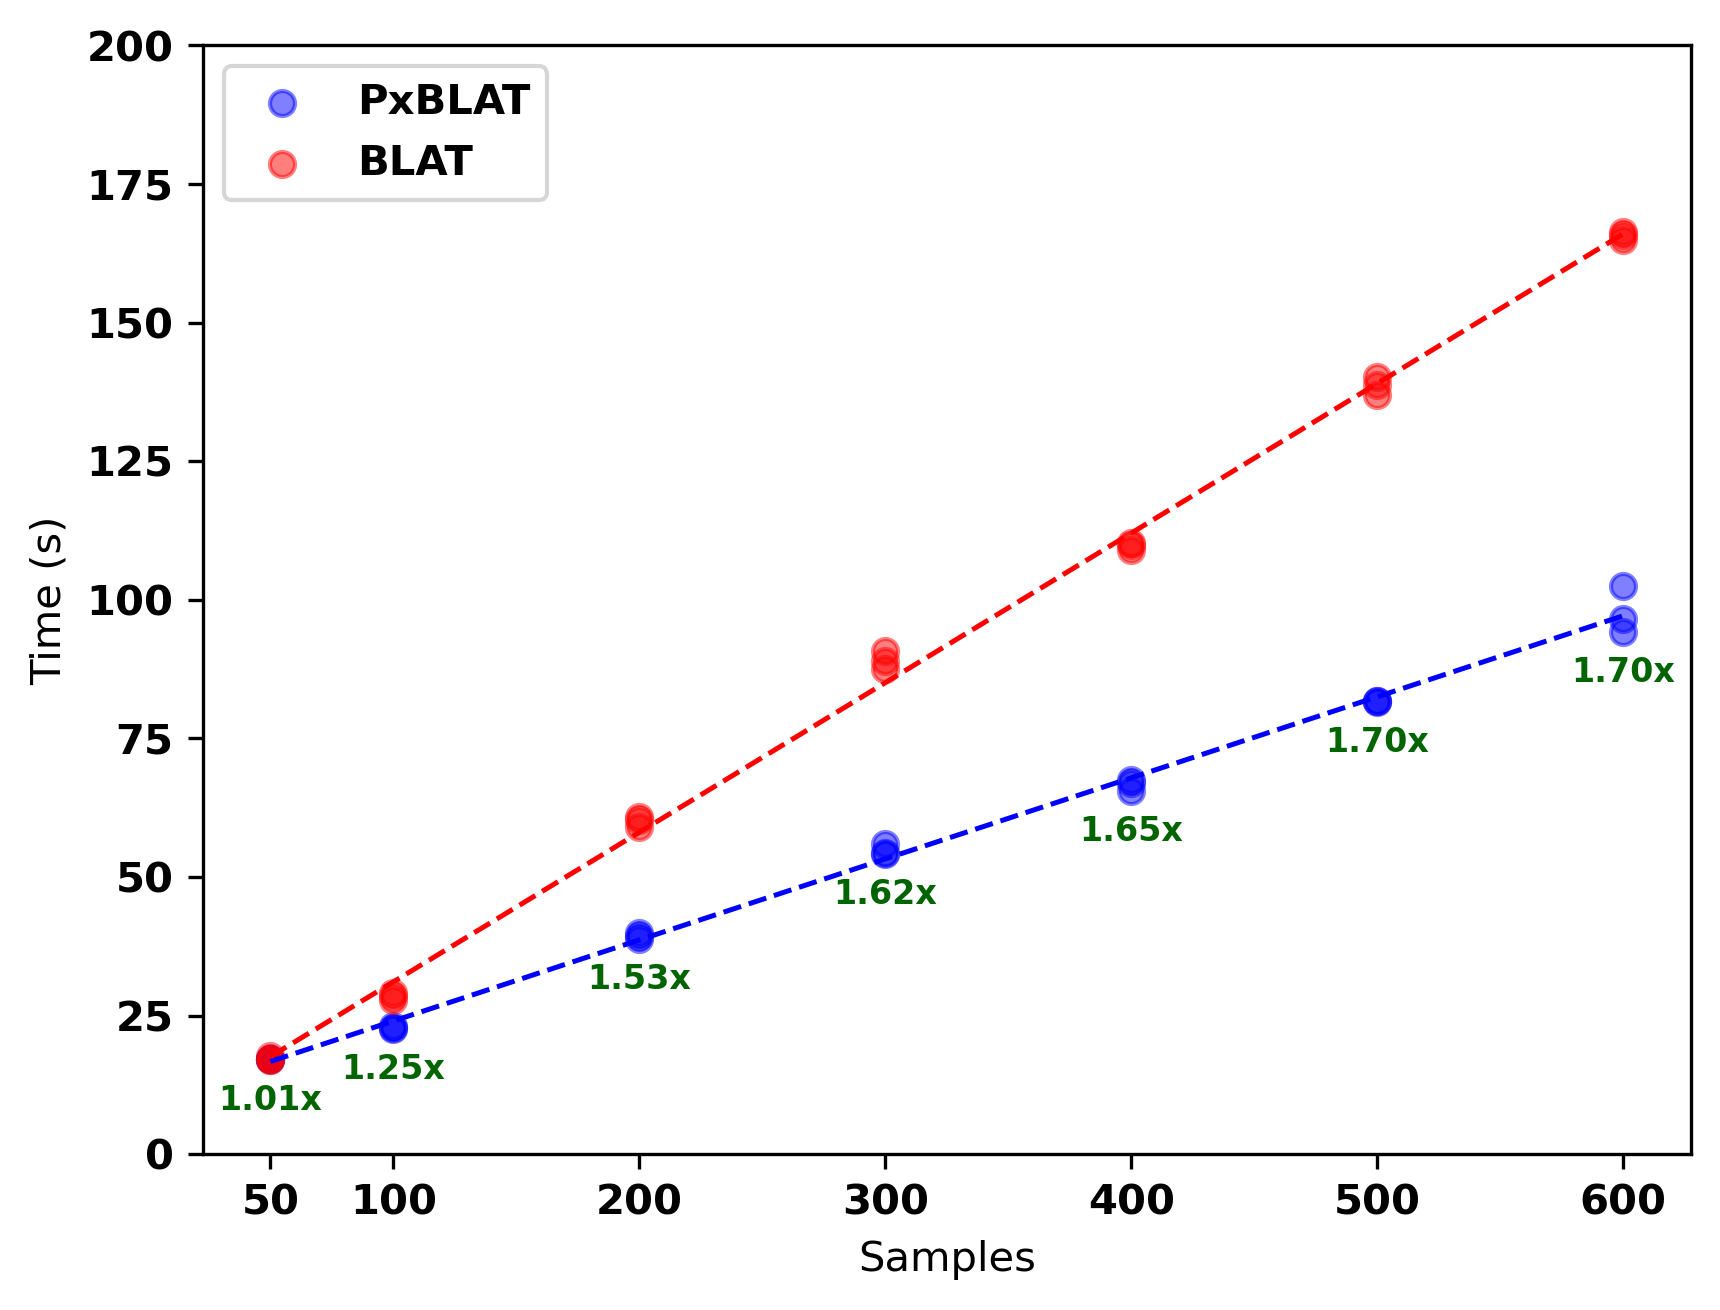
\includegraphics[width=\linewidth]{figures/performance}
	\caption{{\bf Performance comparison between \gls{blat} and \gls{pxblat}.} This figure quantifies the performance of \gls{blat} (indicated by red points) and \gls{pxblat} (indicated by blue points) across various data sets, with the \(x\) axis categorizing the number of samples in the sets and the \(y\) axis detailing the execution time in seconds.
		Each group encapsulates the results of three independent experiments.
		Trend lines, depicted in red for \gls{blat} and blue for \gls{pxblat}, illustrate the general performance pattern for each tool.
		Notably, the green text highlights the speedup achieved by PxBLAT, calculated as the ratio of the execution time (\(\mathrm{time}_\textsubscript{blat} / \mathrm{time}_\textsubscript{pxblat}\)), underscoring the efficiency gains of \gls{pxblat} relative to \gls{blat}.}
	\label{fig:performance}
\end{figure}

In summary, \gls{pxblat} demonstrates significant advantages in terms of execution time reduction and enhanced user experience.
These findings underscore its utility as a substantial improvement over the \gls{blat}, reinforcing its value within the bioinformatics toolkit.

\subsection*{Availability and future directions}

The \gls{pxblat}, along with the source code, is publicly available in the GitHub repository at \url{https://github.com/ylab-hi/pxblat}.
The documentation is available at ReadtheDocs \url{https://pxblat.readthedocs.io/en/latest/}.
The script for benchmarking is available at \emph{tests/test\_result.py} in the repository.
The testing dataset is available at the GitHub repository {\url{https://github.com/ylab-hi/pxblat}.
The path of the testing dataset is \emph{benchmark/fas}.

As we advance \gls{pxblat}, our vision is firmly set on developing a robust, user-oriented tool that dynamically meets the evolving demands of the bioinformatics community.
Our commitment to continuous improvement is guided by insightful user feedback and the latest scientific advancements.
Future enhancements of \gls{pxblat} are directed towards augmenting functionality through the introduction of innovative features and the refinement of existing ones, thereby expanding the tool's adaptability to a diverse range of data types and bioinformatics workflows.

A relentless pursuit of performance optimization remains at the core of our efforts, aiming to significantly enhance efficiency, reduce computational overhead, and streamline the overall user experience.
Additionally, we are committed to the development of comprehensive educational materials, including detailed tutorials, insightful case studies, and best practice guidelines.
Together, these focused endeavors epitomize our dedication to excellence and our aspiration to nurture an inclusive, innovative, and community-driven ecosystem in the field of bioinformatics.

%\section*{Discussion}
%\section*{Conclusion}


\section*{Supporting information}

% Include only the SI item label in the paragraph heading. Use the \nameref{label} command to cite SI items in the text.
%\paragraph*{S1 Fig.}
%\label{S1_Fig}
%{\bf Bold the title sentence.} Add descriptive text after the title of the item (optional).
%
%\paragraph*{S2 Fig.}
%\label{S2_Fig}
%{\bf Lorem ipsum.} Maecenas convallis mauris sit amet sem ultrices gravida. Etiam eget sapien nibh. Sed ac ipsum eget enim egestas ullamcorper nec euismod ligula. Curabitur fringilla pulvinar lectus consectetur pellentesque.
%
%\paragraph*{S1 File.}
%\label{S1_File}
%{\bf Lorem ipsum.}  Maecenas convallis mauris sit amet sem ultrices gravida. Etiam eget sapien nibh. Sed ac ipsum eget enim egestas ullamcorper nec euismod ligula. Curabitur fringilla pulvinar lectus consectetur pellentesque.
%
%\paragraph*{S1 Video.}
%\label{S1_Video}
%{\bf Lorem ipsum.}  Maecenas convallis mauris sit amet sem ultrices gravida. Etiam eget sapien nibh. Sed ac ipsum eget enim egestas ullamcorper nec euismod ligula. Curabitur fringilla pulvinar lectus consectetur pellentesque.
%
%\paragraph*{S1 Appendix.}
%\label{S1_Appendix}
%{\bf Lorem ipsum.} Maecenas convallis mauris sit amet sem ultrices gravida. Etiam eget sapien nibh. Sed ac ipsum eget enim egestas ullamcorper nec euismod ligula. Curabitur fringilla pulvinar lectus consectetur pellentesque.

\paragraph*{S1 Table.}
\label{S1_Table}
{\bf Performance comparison between \gls{pxblat} and \gls{blat}.}
This table illustrates the performance of both \gls{pxblat} and \gls{blat} across data sets containing \num{50},  \num{100}, \num{200}, \num{300}, \num{400}, \num{500}, and \num{600} samples.
For each data set, three independent experiments are conducted to ensure robust performance evaluation.
The efficiency of \gls{pxblat} relative to \gls{blat} is quantified through the speedup metric, calculated as the ratio of the execution time (\(\mathrm{time}_\textsubscript{blat} / \mathrm{time}_\textsubscript{pxblat}\)).
This comparison highlights the computational advantages of \gls{pxblat} in terms of processing speed.

\begin{longtable}{SSSS}
	\toprule
	{Samples} & {PxBLAT (s)} & {BLAT (s)} & {Speedup} \\
	\midrule
	\endfirsthead
	\toprule
	{Samples} & {PxBLAT (s)} & {BLAT (s)} & {Speedup} \\
	\midrule
	\endhead
	\midrule
	\multicolumn{4}{r}{Continued on next page}        \\
	\midrule
	\endfoot
	\bottomrule
	\endlastfoot
	50        & 17.102400    & 17.034500  & 0.996030  \\
	50        & 17.092300    & 17.006900  & 0.995004  \\
	50        & 17.098200    & 17.722700  & 1.036524  \\
	100       & 22.749400    & 28.613600  & 1.257774  \\
	100       & 23.117700    & 29.097000  & 1.258646  \\
	100       & 22.534500    & 27.896400  & 1.237942  \\
	200       & 39.307500    & 59.027200  & 1.501678  \\
	200       & 38.859800    & 60.203200  & 1.549241  \\
	200       & 39.804700    & 60.873500  & 1.529304  \\
	300       & 55.893000    & 90.681000  & 1.622404  \\
	300       & 54.335900    & 88.877800  & 1.635710  \\
	300       & 54.154300    & 87.464200  & 1.615092  \\
	400       & 65.502000    & 110.204600 & 1.682462  \\
	400       & 67.017500    & 109.058900 & 1.627320  \\
	400       & 67.456100    & 109.789200 & 1.627565  \\
	500       & 81.555000    & 140.131900 & 1.718250  \\
	500       & 81.767500    & 138.657600 & 1.695754  \\
	500       & 81.730400    & 137.019200 & 1.676478  \\
	600       & 96.620400    & 165.867600 & 1.716693  \\
	600       & 102.548000   & 164.930200 & 1.608322  \\
	600       & 94.208100    & 166.379300 & 1.766083  \\
\end{longtable}

\paragraph*{S2 Table.}
\label{S2_Table}
{\bf \gls{hsp} comparison between \gls{pxblat} and \gls{blat}.}
This table, including \num{600} samples in total, presents a comparison of the \glspl{hsp} generated by \gls{blat} and \gls{pxblat} for each sample.
The column Sample lists the name of the sample, and the columns \gls{blat} and \gls{pxblat}, respectively denote the number of \glspl{hsp} generated by \gls{blat} and \gls{pxblat}.

\begin{longtable}{lSS}
	%    \caption{HSP Comparison between BLAT and PxBLAT} \label{tab:cmp} \\
	\toprule
	Sample                  & {BLAT} & {PxBLAT} \\
	\midrule
	\endfirsthead
	%	\caption[]{\gls{hsp} Comparison between BLAT and PxBLAT} \\
	\toprule
	Sample                  & {BLAT} & {PxBLAT} \\
	\midrule
	\endhead
	\midrule
	\multicolumn{3}{r}{Continued on next page}  \\
	\midrule
	\endfoot
	\bottomrule
	\endlastfoot
	chr20-11648866-11650925 & 130    & 130      \\
	chr20-29850079-29852595 & 1      & 1        \\
	chr20-7493878-7496145   & 26     & 26       \\
	chr20-30152074-30153892 & 3      & 3        \\
	chr20-1140095-1141788   & 22     & 22       \\
	chr20-17520690-17523557 & 14     & 14       \\
	chr20-41374266-41376291 & 12     & 12       \\
	chr20-63240773-63243242 & 64     & 64       \\
	chr20-59286740-59288091 & 13     & 13       \\
	chr20-8061734-8063508   & 10     & 10       \\
	chr20-34429296-34431248 & 41     & 41       \\
	chr20-27977914-27979241 & 22     & 22       \\
	chr20-11695455-11697457 & 20     & 20       \\
	chr20-41792348-41794797 & 131    & 131      \\
	chr20-25858004-25860351 & 37     & 37       \\
	chr20-31404034-31407027 & 25     & 25       \\
	chr20-15852904-15855300 & 65     & 65       \\
	chr20-29917054-29919227 & 18     & 18       \\
	chr20-45175162-45177033 & 2      & 2        \\
	chr20-43937342-43939507 & 58     & 58       \\
	chr20-17073859-17076499 & 48     & 48       \\
	chr20-19823346-19824950 & 32     & 32       \\
	chr20-28295597-28298301 & 23     & 23       \\
	chr20-15826504-15829187 & 26     & 26       \\
	chr20-54683378-54684991 & 47     & 47       \\
	chr20-55475241-55476377 & 18     & 18       \\
	chr20-57949934-57952283 & 74     & 74       \\
	chr20-14442978-14444604 & 35     & 35       \\
	chr20-51293808-51295630 & 38     & 38       \\
	chr20-49194155-49196823 & 165    & 165      \\
	chr20-34696351-34697788 & 43     & 43       \\
	chr20-16044321-16045712 & 48     & 48       \\
	chr20-45309757-45312553 & 39     & 39       \\
	chr20-21063232-21065145 & 26     & 26       \\
	chr20-434138-436331     & 174    & 174      \\
	chr20-62110486-62112604 & 167    & 167      \\
	chr20-15866914-15868171 & 15     & 15       \\
	chr20-62343940-62345043 & 69     & 69       \\
	chr20-37168356-37170160 & 34     & 34       \\
	chr20-15699683-15701260 & 15     & 15       \\
	chr20-44826183-44827333 & 152    & 152      \\
	chr20-41538435-41540074 & 43     & 43       \\
	chr20-56032843-56034378 & 18     & 18       \\
	chr20-36813618-36816516 & 21     & 21       \\
	chr20-18637848-18640751 & 68     & 68       \\
	chr20-56294086-56296598 & 27     & 27       \\
	chr20-19514094-19515343 & 2      & 2        \\
	chr20-33893321-33895564 & 126    & 126      \\
	chr20-22282380-22283429 & 4      & 4        \\
	chr20-39910629-39912740 & 84     & 84       \\
	chr20-40898874-40901542 & 27     & 27       \\
	chr20-7536153-7537696   & 15     & 15       \\
	chr20-4818626-4819858   & 60     & 60       \\
	chr20-64316707-64319236 & 24     & 24       \\
	chr20-2960440-2961833   & 119    & 119      \\
	chr20-2519249-2521676   & 46     & 46       \\
	chr20-11596878-11599706 & 68     & 68       \\
	chr20-30829536-30831739 & 16     & 16       \\
	chr20-45188854-45190558 & 3      & 3        \\
	chr20-47238745-47241145 & 14     & 14       \\
	chr20-10538965-10540232 & 83     & 83       \\
	chr20-11996320-11998343 & 87     & 87       \\
	chr20-23440919-23442976 & 47     & 47       \\
	chr20-22451495-22453568 & 4      & 4        \\
	chr20-39709672-39711911 & 23     & 23       \\
	chr20-29782708-29784088 & 8      & 8        \\
	chr20-7911434-7913178   & 9      & 9        \\
	chr20-1508550-1511129   & 193    & 193      \\
	chr20-41451172-41452837 & 6      & 6        \\
	chr20-4003988-4006545   & 29     & 29       \\
	chr20-10921197-10923149 & 5      & 5        \\
	chr20-36789016-36790500 & 186    & 186      \\
	chr20-9309222-9310479   & 157    & 157      \\
	chr20-52532795-52534564 & 9      & 9        \\
	chr20-42081563-42082983 & 4      & 4        \\
	chr20-12605319-12606971 & 2      & 2        \\
	chr20-29389010-29390598 & 149    & 149      \\
	chr20-8128132-8130266   & 170    & 170      \\
	chr20-11399422-11401237 & 12     & 12       \\
	chr20-33251227-33252414 & 2      & 2        \\
	chr20-3342256-3343645   & 92     & 92       \\
	chr20-38869283-38872088 & 60     & 60       \\
	chr20-7649152-7650444   & 60     & 60       \\
	chr20-13021673-13023769 & 58     & 58       \\
	chr20-3971117-3972667   & 32     & 32       \\
	chr20-26232703-26234929 & 61     & 61       \\
	chr20-23063517-23064745 & 7      & 7        \\
	chr20-39079691-39080763 & 26     & 26       \\
	chr20-23882126-23884119 & 92     & 92       \\
	chr20-3170215-3172728   & 44     & 44       \\
	chr20-49421601-49423499 & 35     & 35       \\
	chr20-55380779-55383730 & 204    & 204      \\
	chr20-45794728-45796900 & 164    & 164      \\
	chr20-15159613-15161221 & 9      & 9        \\
	chr20-62378279-62380174 & 184    & 184      \\
	chr20-6934771-6936584   & 116    & 116      \\
	chr20-59538484-59541329 & 8      & 8        \\
	chr20-43661982-43664714 & 26     & 26       \\
	chr20-36707842-36709247 & 85     & 85       \\
	chr20-33898085-33900435 & 65     & 65       \\
	chr20-18062688-18064265 & 46     & 46       \\
	chr20-29490152-29491491 & 23     & 23       \\
	chr20-30806959-30809757 & 0      & 0        \\
	chr20-11837593-11840377 & 40     & 40       \\
	chr20-28934655-28937276 & 1      & 1        \\
	chr20-7689471-7691553   & 18     & 18       \\
	chr20-1746811-1749803   & 9      & 9        \\
	chr20-1261408-1262588   & 16     & 16       \\
	chr20-5757029-5759548   & 29     & 29       \\
	chr20-5361957-5364278   & 107    & 107      \\
	chr20-37305589-37308001 & 21     & 21       \\
	chr20-53702835-53705300 & 148    & 148      \\
	chr20-7447290-7449191   & 16     & 16       \\
	chr20-36626015-36629010 & 150    & 150      \\
	chr20-48184357-48185678 & 2      & 2        \\
	chr20-4634043-4636057   & 9      & 9        \\
	chr20-21292878-21295830 & 179    & 179      \\
	chr20-52551672-52553086 & 7      & 7        \\
	chr20-55410142-55411547 & 55     & 55       \\
	chr20-15164296-15166007 & 21     & 21       \\
	chr20-60294852-60297789 & 197    & 197      \\
	chr20-47112993-47114241 & 38     & 38       \\
	chr20-33645643-33648541 & 62     & 62       \\
	chr20-57099663-57101555 & 91     & 91       \\
	chr20-32443012-32444528 & 1      & 1        \\
	chr20-54597242-54598325 & 31     & 31       \\
	chr20-28168758-28171348 & 20     & 20       \\
	chr20-14255274-14256294 & 211    & 211      \\
	chr20-22858139-22859797 & 8      & 8        \\
	chr20-42977157-42978222 & 11     & 11       \\
	chr20-3890553-3891667   & 46     & 46       \\
	chr20-10043505-10044872 & 33     & 33       \\
	chr20-47292153-47293840 & 50     & 50       \\
	chr20-30056354-30058719 & 0      & 0        \\
	chr20-23406092-23408775 & 15     & 15       \\
	chr20-44245002-44246392 & 36     & 36       \\
	chr20-30999482-31002350 & 1      & 1        \\
	chr20-11990150-11991239 & 3      & 3        \\
	chr20-3810992-3812466   & 197    & 197      \\
	chr20-26419101-26422061 & 0      & 0        \\
	chr20-22091287-22094021 & 119    & 119      \\
	chr20-47477509-47479589 & 59     & 59       \\
	chr20-13750647-13753070 & 44     & 44       \\
	chr20-61483678-61484972 & 2      & 2        \\
	chr20-57584630-57586794 & 13     & 13       \\
	chr20-17904728-17906925 & 34     & 34       \\
	chr20-28086098-28087474 & 19     & 19       \\
	chr20-21317295-21318548 & 51     & 51       \\
	chr20-42758324-42759488 & 193    & 193      \\
	chr20-23580801-23581810 & 23     & 23       \\
	chr20-58929386-58930631 & 22     & 22       \\
	chr20-6605062-6607136   & 79     & 79       \\
	chr20-32987534-32989963 & 169    & 169      \\
	chr20-22493043-22494805 & 22     & 22       \\
	chr20-54190709-54192035 & 24     & 24       \\
	chr20-48343887-48346044 & 2      & 2        \\
	chr20-10262876-10265171 & 189    & 189      \\
	chr20-35374558-35376267 & 67     & 67       \\
	chr20-39018648-39021540 & 83     & 83       \\
	chr20-37785924-37788264 & 202    & 202      \\
	chr20-64334961-64337760 & 0      & 0        \\
	chr20-12575681-12578297 & 14     & 14       \\
	chr20-23374273-23375283 & 1      & 1        \\
	chr20-14278920-14280350 & 40     & 40       \\
	chr20-42778102-42780755 & 9      & 9        \\
	chr20-52810557-52811573 & 83     & 83       \\
	chr20-52564945-52566606 & 22     & 22       \\
	chr20-10598821-10601808 & 32     & 32       \\
	chr20-1172826-1175431   & 87     & 87       \\
	chr20-3347653-3350627   & 44     & 44       \\
	chr20-64176870-64179763 & 43     & 43       \\
	chr20-42829128-42830258 & 100    & 100      \\
	chr20-40623645-40625957 & 187    & 187      \\
	chr20-27009229-27011878 & 24     & 24       \\
	chr20-14732847-14734481 & 95     & 95       \\
	chr20-12698635-12699679 & 2      & 2        \\
	chr20-13328590-13330614 & 13     & 13       \\
	chr20-22912395-22915205 & 12     & 12       \\
	chr20-35339375-35342113 & 48     & 48       \\
	chr20-19431509-19433187 & 28     & 28       \\
	chr20-28727730-28729750 & 16     & 16       \\
	chr20-39515806-39517118 & 2      & 2        \\
	chr20-21857448-21859310 & 209    & 209      \\
	chr20-44751640-44753567 & 19     & 19       \\
	chr20-47371415-47374127 & 45     & 45       \\
	chr20-24140371-24142959 & 6      & 6        \\
	chr20-54083025-54084528 & 41     & 41       \\
	chr20-51775800-51777458 & 46     & 46       \\
	chr20-59400225-59402632 & 30     & 30       \\
	chr20-57144627-57147621 & 47     & 47       \\
	chr20-17690928-17692128 & 6      & 6        \\
	chr20-31238605-31240139 & 4      & 4        \\
	chr20-29259215-29262074 & 4      & 4        \\
	chr20-39132690-39134466 & 34     & 34       \\
	chr20-44674003-44676622 & 31     & 31       \\
	chr20-34435089-34436815 & 13     & 13       \\
	chr20-11085268-11087065 & 27     & 27       \\
	chr20-42010931-42012642 & 10     & 10       \\
	chr20-7483012-7484115   & 1      & 1        \\
	chr20-39873233-39875635 & 207    & 207      \\
	chr20-32029134-32032031 & 93     & 93       \\
	chr20-38052616-38054138 & 32     & 32       \\
	chr20-2602976-2605324   & 19     & 19       \\
	chr20-42169915-42172757 & 15     & 15       \\
	chr20-62125729-62128471 & 19     & 19       \\
	chr20-2162753-2164165   & 5      & 5        \\
	chr20-34630972-34632436 & 113    & 113      \\
	chr20-6611620-6614440   & 152    & 152      \\
	chr20-19300360-19302642 & 6      & 6        \\
	chr20-25189802-25191365 & 154    & 154      \\
	chr20-15951964-15953450 & 26     & 26       \\
	chr20-47285001-47287102 & 52     & 52       \\
	chr20-22548369-22549974 & 9      & 9        \\
	chr20-24725480-24727693 & 52     & 52       \\
	chr20-55633941-55636718 & 5      & 5        \\
	chr20-30324027-30326285 & 30     & 30       \\
	chr20-34789703-34791591 & 27     & 27       \\
	chr20-22886111-22887126 & 5      & 5        \\
	chr20-52373722-52374925 & 52     & 52       \\
	chr20-62594615-62596270 & 61     & 61       \\
	chr20-23567798-23569994 & 5      & 5        \\
	chr20-52746782-52748970 & 26     & 26       \\
	chr20-63919107-63920159 & 20     & 20       \\
	chr20-37603411-37606081 & 21     & 21       \\
	chr20-45549091-45551404 & 167    & 167      \\
	chr20-24122821-24124880 & 2      & 2        \\
	chr20-39384970-39386746 & 47     & 47       \\
	chr20-56953750-56954962 & 11     & 11       \\
	chr20-27265832-27268665 & 27     & 27       \\
	chr20-989008-991475     & 96     & 96       \\
	chr20-13233506-13234845 & 9      & 9        \\
	chr20-30767954-30769153 & 0      & 0        \\
	chr20-54079315-54081921 & 56     & 56       \\
	chr20-22276591-22279281 & 202    & 202      \\
	chr20-32344273-32347087 & 26     & 26       \\
	chr20-14761627-14763228 & 15     & 15       \\
	chr20-24471803-24474607 & 7      & 7        \\
	chr20-22305788-22308754 & 43     & 43       \\
	chr20-63927315-63929626 & 54     & 54       \\
	chr20-33534721-33537439 & 158    & 158      \\
	chr20-53020990-53022920 & 33     & 33       \\
	chr20-44701412-44703325 & 34     & 34       \\
	chr20-63523339-63524524 & 190    & 190      \\
	chr20-39750571-39752199 & 50     & 50       \\
	chr20-47879542-47880820 & 162    & 162      \\
	chr20-12949055-12950079 & 1      & 1        \\
	chr20-37737796-37740734 & 26     & 26       \\
	chr20-17600492-17603407 & 68     & 68       \\
	chr20-40848143-40849212 & 2      & 2        \\
	chr20-33135173-33136880 & 131    & 131      \\
	chr20-39118192-39119260 & 4      & 4        \\
	chr20-27690465-27692366 & 23     & 23       \\
	chr20-37858061-37860321 & 49     & 49       \\
	chr20-12405605-12407882 & 6      & 6        \\
	chr20-57386121-57387852 & 70     & 70       \\
	chr20-34902889-34905611 & 39     & 39       \\
	chr20-52070637-52073331 & 35     & 35       \\
	chr20-40779660-40781751 & 47     & 47       \\
	chr20-31098450-31100717 & 3      & 3        \\
	chr20-29969458-29971235 & 18     & 18       \\
	chr20-13789470-13791842 & 152    & 152      \\
	chr20-26814485-26817257 & 22     & 22       \\
	chr20-40740691-40742983 & 29     & 29       \\
	chr20-49955693-49958425 & 183    & 183      \\
	chr20-37813305-37814584 & 9      & 9        \\
	chr20-18255943-18258048 & 64     & 64       \\
	chr20-63109432-63111043 & 34     & 34       \\
	chr20-14211039-14213272 & 9      & 9        \\
	chr20-17100441-17103140 & 9      & 9        \\
	chr20-2866996-2869328   & 38     & 38       \\
	chr20-53703835-53705398 & 158    & 158      \\
	chr20-51431118-51433743 & 56     & 56       \\
	chr20-6192786-6193790   & 196    & 196      \\
	chr20-10748356-10751019 & 35     & 35       \\
	chr20-33974548-33976407 & 44     & 44       \\
	chr20-32270385-32273111 & 20     & 20       \\
	chr20-36902282-36904506 & 28     & 28       \\
	chr20-198832-201190     & 40     & 40       \\
	chr20-7927314-7928574   & 27     & 27       \\
	chr20-17899461-17900502 & 58     & 58       \\
	chr20-11120841-11122366 & 23     & 23       \\
	chr20-59407661-59409193 & 27     & 27       \\
	chr20-35649824-35652625 & 5      & 5        \\
	chr20-30688628-30690580 & 48     & 48       \\
	chr20-49466264-49467309 & 5      & 5        \\
	chr20-63692672-63694078 & 2      & 2        \\
	chr20-12570747-12573421 & 5      & 5        \\
	chr20-8512304-8514491   & 20     & 20       \\
	chr20-24204303-24205314 & 2      & 2        \\
	chr20-11639430-11641175 & 20     & 20       \\
	chr20-26938330-26940788 & 24     & 24       \\
	chr20-17587799-17589501 & 209    & 209      \\
	chr20-26384682-26386149 & 23     & 23       \\
	chr20-46308421-46310414 & 41     & 41       \\
	chr20-30072951-30074554 & 0      & 0        \\
	chr20-44079162-44081096 & 23     & 23       \\
	chr20-21475551-21476686 & 50     & 50       \\
	chr20-13972488-13974627 & 44     & 44       \\
	chr20-45697903-45699479 & 88     & 88       \\
	chr20-24838480-24839925 & 11     & 11       \\
	chr20-7742386-7745111   & 4      & 4        \\
	chr20-56522851-56524815 & 12     & 12       \\
	chr20-22497057-22499773 & 16     & 16       \\
	chr20-51998729-52000293 & 22     & 22       \\
	chr20-38767581-38768689 & 5      & 5        \\
	chr20-19863311-19865822 & 56     & 56       \\
	chr20-9295230-9297764   & 226    & 226      \\
	chr20-15012779-15015584 & 8      & 8        \\
	chr20-5041846-5044587   & 56     & 56       \\
	chr20-580210-582022     & 35     & 35       \\
	chr20-15328579-15331324 & 42     & 42       \\
	chr20-49481967-49483214 & 17     & 17       \\
	chr20-5260817-5262044   & 5      & 5        \\
	chr20-23340929-23343084 & 102    & 102      \\
	chr20-2269716-2270774   & 189    & 189      \\
	chr20-46399947-46401667 & 31     & 31       \\
	chr20-10815100-10817410 & 32     & 32       \\
	chr20-45864818-45866440 & 53     & 53       \\
	chr20-45489949-45492069 & 35     & 35       \\
	chr20-21302718-21304312 & 1      & 1        \\
	chr20-9931834-9933992   & 5      & 5        \\
	chr20-56295194-56296721 & 5      & 5        \\
	chr20-38225781-38227971 & 18     & 18       \\
	chr20-18585659-18587381 & 35     & 35       \\
	chr20-16940912-16942721 & 39     & 39       \\
	chr20-3758200-3759977   & 4      & 4        \\
	chr20-11807056-11808124 & 3      & 3        \\
	chr20-127575-129488     & 93     & 93       \\
	chr20-40755444-40756701 & 5      & 5        \\
	chr20-21011682-21013735 & 2      & 2        \\
	chr20-10119043-10120171 & 59     & 59       \\
	chr20-1313128-1315640   & 18     & 18       \\
	chr20-11712977-11715178 & 142    & 142      \\
	chr20-34597997-34600726 & 28     & 28       \\
	chr20-53048517-53050101 & 29     & 29       \\
	chr20-15161566-15163488 & 8      & 8        \\
	chr20-15137364-15139959 & 203    & 203      \\
	chr20-60342420-60345056 & 94     & 94       \\
	chr20-55169861-55170982 & 156    & 156      \\
	chr20-24314101-24316265 & 27     & 27       \\
	chr20-53183314-53186148 & 16     & 16       \\
	chr20-43887385-43889661 & 75     & 75       \\
	chr20-59470391-59471545 & 1      & 1        \\
	chr20-53159093-53161302 & 35     & 35       \\
	chr20-5895129-5896312   & 26     & 26       \\
	chr20-25292499-25293803 & 3      & 3        \\
	chr20-34161145-34162369 & 41     & 41       \\
	chr20-45868564-45870103 & 74     & 74       \\
	chr20-4887453-4889888   & 3      & 3        \\
	chr20-39559840-39561722 & 9      & 9        \\
	chr20-33221436-33223116 & 56     & 56       \\
	chr20-755464-758088     & 35     & 35       \\
	chr20-1111176-1112831   & 46     & 46       \\
	chr20-2802607-2803838   & 36     & 36       \\
	chr20-38997152-38999498 & 22     & 22       \\
	chr20-5049946-5052675   & 35     & 35       \\
	chr20-48767423-48769196 & 48     & 48       \\
	chr20-2659893-2661452   & 56     & 56       \\
	chr20-49121260-49124086 & 21     & 21       \\
	chr20-54247731-54250009 & 75     & 75       \\
	chr20-8334685-8337480   & 34     & 34       \\
	chr20-26427340-26428991 & 0      & 0        \\
	chr20-1762478-1764560   & 46     & 46       \\
	chr20-53286968-53289954 & 23     & 23       \\
	chr20-23613637-23615158 & 53     & 53       \\
	chr20-7135001-7136753   & 88     & 88       \\
	chr20-59872605-59875175 & 5      & 5        \\
	chr20-33944307-33946354 & 27     & 27       \\
	chr20-29344297-29347205 & 8      & 8        \\
	chr20-28334593-28336360 & 22     & 22       \\
	chr20-49230825-49232042 & 66     & 66       \\
	chr20-48044237-48045631 & 3      & 3        \\
	chr20-26227485-26229228 & 5      & 5        \\
	chr20-26487906-26489572 & 25     & 25       \\
	chr20-11596974-11599728 & 65     & 65       \\
	chr20-45661385-45663135 & 194    & 194      \\
	chr20-23562380-23564047 & 2      & 2        \\
	chr20-5735736-5738602   & 12     & 12       \\
	chr20-31727237-31729024 & 39     & 39       \\
	chr20-36152090-36154966 & 151    & 151      \\
	chr20-1018906-1020553   & 11     & 11       \\
	chr20-9821106-9823172   & 75     & 75       \\
	chr20-52034533-52037144 & 85     & 85       \\
	chr20-15008181-15010280 & 66     & 66       \\
	chr20-41851737-41853531 & 6      & 6        \\
	chr20-29408974-29411107 & 20     & 20       \\
	chr20-10955881-10957008 & 1      & 1        \\
	chr20-8970270-8971572   & 18     & 18       \\
	chr20-2350436-2352589   & 200    & 200      \\
	chr20-35494115-35496325 & 37     & 37       \\
	chr20-16994461-16996880 & 203    & 203      \\
	chr20-1121638-1123536   & 20     & 20       \\
	chr20-10539946-10542788 & 76     & 76       \\
	chr20-31981394-31984035 & 24     & 24       \\
	chr20-31059406-31062015 & 9      & 9        \\
	chr20-23005241-23006490 & 85     & 85       \\
	chr20-27678668-27680740 & 22     & 22       \\
	chr20-23089029-23090440 & 1      & 1        \\
	chr20-18766639-18768846 & 74     & 74       \\
	chr20-35270491-35271927 & 24     & 24       \\
	chr20-32671767-32673927 & 46     & 46       \\
	chr20-5469364-5470405   & 1      & 1        \\
	chr20-44586665-44588074 & 3      & 3        \\
	chr20-19751371-19752469 & 50     & 50       \\
	chr20-11475039-11477338 & 4      & 4        \\
	chr20-52930875-52933353 & 52     & 52       \\
	chr20-23941121-23942933 & 189    & 189      \\
	chr20-10612667-10615654 & 16     & 16       \\
	chr20-39220431-39222072 & 6      & 6        \\
	chr20-24056618-24059198 & 190    & 190      \\
	chr20-63753892-63756615 & 196    & 196      \\
	chr20-64298054-64301011 & 16     & 16       \\
	chr20-43632072-43634462 & 46     & 46       \\
	chr20-29402266-29403661 & 49     & 49       \\
	chr20-34611441-34612505 & 39     & 39       \\
	chr20-16219627-16222599 & 19     & 19       \\
	chr20-47623287-47624373 & 18     & 18       \\
	chr20-37572653-37574987 & 20     & 20       \\
	chr20-57328038-57329145 & 159    & 159      \\
	chr20-54255861-54257299 & 11     & 11       \\
	chr20-17523656-17525455 & 3      & 3        \\
	chr20-3054439-3055812   & 26     & 26       \\
	chr20-51095602-51096740 & 8      & 8        \\
	chr20-26295259-26296843 & 6      & 6        \\
	chr20-16956946-16959866 & 4      & 4        \\
	chr20-59871467-59873730 & 18     & 18       \\
	chr20-12972124-12973571 & 9      & 9        \\
	chr20-64187505-64190371 & 7      & 7        \\
	chr20-20036801-20038441 & 54     & 54       \\
	chr20-52361579-52363650 & 49     & 49       \\
	chr20-48763637-48765211 & 21     & 21       \\
	chr20-29272745-29274078 & 3      & 3        \\
	chr20-6596603-6597647   & 1      & 1        \\
	chr20-25092945-25094053 & 38     & 38       \\
	chr20-23976043-23978934 & 34     & 34       \\
	chr20-33528290-33530524 & 183    & 183      \\
	chr20-45968564-45971166 & 41     & 41       \\
	chr20-29195839-29197450 & 17     & 17       \\
	chr20-12991634-12993772 & 18     & 18       \\
	chr20-7287285-7289523   & 45     & 45       \\
	chr20-12780972-12782351 & 20     & 20       \\
	chr20-17273569-17275885 & 46     & 46       \\
	chr20-53404329-53405379 & 8      & 8        \\
	chr20-32199416-32201827 & 159    & 159      \\
	chr20-56899277-56900938 & 64     & 64       \\
	chr20-21026086-21027263 & 198    & 198      \\
	chr20-29495766-29497356 & 5      & 5        \\
	chr20-46509725-46510768 & 176    & 176      \\
	chr20-44370323-44372070 & 36     & 36       \\
	chr20-34807421-34810326 & 128    & 128      \\
	chr20-29310629-29312542 & 80     & 80       \\
	chr20-1861413-1862970   & 10     & 10       \\
	chr20-13425759-13427299 & 2      & 2        \\
	chr20-40797946-40799834 & 14     & 14       \\
	chr20-9134988-9136715   & 38     & 38       \\
	chr20-6129194-6130506   & 20     & 20       \\
	chr20-32328850-32331341 & 40     & 40       \\
	chr20-37816931-37818838 & 30     & 30       \\
	chr20-43643216-43645801 & 82     & 82       \\
	chr20-57951819-57954389 & 39     & 39       \\
	chr20-38495333-38497995 & 69     & 69       \\
	chr20-23579562-23580734 & 13     & 13       \\
	chr20-32476687-32477738 & 89     & 89       \\
	chr20-46657968-46660258 & 17     & 17       \\
	chr20-44029371-44030373 & 1      & 1        \\
	chr20-19040746-19042992 & 24     & 24       \\
	chr20-41547378-41548428 & 5      & 5        \\
	chr20-31338848-31340507 & 33     & 33       \\
	chr20-50733531-50736468 & 30     & 30       \\
	chr20-23264110-23266210 & 46     & 46       \\
	chr20-59975068-59976189 & 25     & 25       \\
	chr20-40116512-40117628 & 2      & 2        \\
	chr20-34348380-34351135 & 191    & 191      \\
	chr20-53857114-53859581 & 90     & 90       \\
	chr20-24510328-24512009 & 40     & 40       \\
	chr20-2400648-2401902   & 51     & 51       \\
	chr20-41951417-41953958 & 8      & 8        \\
	chr20-10519505-10521311 & 173    & 173      \\
	chr20-38229341-38232239 & 39     & 39       \\
	chr20-1961461-1962512   & 4      & 4        \\
	chr20-4493702-4496293   & 164    & 164      \\
	chr20-39058190-39059640 & 65     & 65       \\
	chr20-11840010-11842763 & 159    & 159      \\
	chr20-51385931-51387697 & 2      & 2        \\
	chr20-32743241-32746228 & 61     & 61       \\
	chr20-36043748-36044868 & 4      & 4        \\
	chr20-47940674-47941937 & 27     & 27       \\
	chr20-22906294-22908788 & 8      & 8        \\
	chr20-46563742-46565560 & 42     & 42       \\
	chr20-34970963-34972526 & 22     & 22       \\
	chr20-46825075-46827145 & 11     & 11       \\
	chr20-6428315-6430827   & 188    & 188      \\
	chr20-42217777-42219934 & 16     & 16       \\
	chr20-19913134-19914585 & 34     & 34       \\
	chr20-37718004-37720318 & 152    & 152      \\
	chr20-51873445-51875614 & 85     & 85       \\
	chr20-21185966-21187683 & 41     & 41       \\
	chr20-36715891-36717659 & 71     & 71       \\
	chr20-25706788-25709614 & 123    & 123      \\
	chr20-50918346-50919658 & 55     & 55       \\
	chr20-19216584-19217715 & 110    & 110      \\
	chr20-60913180-60914343 & 27     & 27       \\
	chr20-40445916-40447302 & 2      & 2        \\
	chr20-39471792-39473038 & 200    & 200      \\
	chr20-36763453-36764650 & 82     & 82       \\
	chr20-58906803-58909272 & 170    & 170      \\
	chr20-24358042-24359864 & 9      & 9        \\
	chr20-5054910-5055935   & 113    & 113      \\
	chr20-39718409-39719767 & 60     & 60       \\
	chr20-48995874-48997427 & 47     & 47       \\
	chr20-11060084-11062288 & 61     & 61       \\
	chr20-3041121-3043902   & 46     & 46       \\
	chr20-11729530-11731335 & 4      & 4        \\
	chr20-6876021-6878545   & 44     & 44       \\
	chr20-60459034-60461357 & 22     & 22       \\
	chr20-50558110-50560711 & 68     & 68       \\
	chr20-1551191-1553332   & 2      & 2        \\
	chr20-23189149-23191563 & 50     & 50       \\
	chr20-46682255-46683957 & 5      & 5        \\
	chr20-46693319-46694364 & 56     & 56       \\
	chr20-50170226-50172189 & 11     & 11       \\
	chr20-63698924-63701762 & 5      & 5        \\
	chr20-62756096-62757580 & 69     & 69       \\
	chr20-55371351-55373202 & 30     & 30       \\
	chr20-61650045-61652414 & 3      & 3        \\
	chr20-33091750-33093858 & 24     & 24       \\
	chr20-61216684-61218692 & 7      & 7        \\
	chr20-47978091-47980293 & 85     & 85       \\
	chr20-16870384-16872626 & 14     & 14       \\
	chr20-55265469-55267149 & 6      & 6        \\
	chr20-42713744-42715938 & 38     & 38       \\
	chr20-20608914-20611491 & 36     & 36       \\
	chr20-59966328-59967826 & 57     & 57       \\
	chr20-29829808-29831310 & 8      & 8        \\
	chr20-55321262-55323731 & 34     & 34       \\
	chr20-38905281-38906801 & 57     & 57       \\
	chr20-5081835-5084428   & 35     & 35       \\
	chr20-12399681-12402397 & 19     & 19       \\
	chr20-15787670-15789236 & 10     & 10       \\
	chr20-61849267-61851471 & 112    & 112      \\
	chr20-42224821-42226456 & 8      & 8        \\
	chr20-2200973-2202184   & 2      & 2        \\
	chr20-44016368-44018208 & 138    & 138      \\
	chr20-42732744-42735046 & 2      & 2        \\
	chr20-8901543-8903090   & 37     & 37       \\
	chr20-33361770-33363718 & 16     & 16       \\
	chr20-60319529-60322435 & 17     & 17       \\
	chr20-9417083-9419320   & 19     & 19       \\
	chr20-47368389-47371245 & 181    & 181      \\
	chr20-49829087-49831301 & 97     & 97       \\
	chr20-45577205-45579659 & 30     & 30       \\
	chr20-9885847-9887724   & 4      & 4        \\
	chr20-34086336-34087450 & 25     & 25       \\
	chr20-12690873-12693547 & 25     & 25       \\
	chr20-61265483-61267506 & 31     & 31       \\
	chr20-60767473-60770234 & 21     & 21       \\
	chr20-37096290-37097735 & 46     & 46       \\
	chr20-19806699-19808018 & 39     & 39       \\
	chr20-5383554-5385658   & 41     & 41       \\
	chr20-46475786-46476831 & 62     & 62       \\
	chr20-35346166-35347602 & 30     & 30       \\
	chr20-39431060-39432816 & 28     & 28       \\
	chr20-50643697-50644883 & 205    & 205      \\
	chr20-22403148-22404794 & 15     & 15       \\
	chr20-26331430-26334030 & 3      & 3        \\
	chr20-14375436-14376511 & 196    & 196      \\
	chr20-32839818-32840903 & 124    & 124      \\
	chr20-20727967-20730763 & 59     & 59       \\
	chr20-25447522-25449068 & 21     & 21       \\
	chr20-52094840-52096680 & 143    & 143      \\
	chr20-21563954-21565882 & 146    & 146      \\
	chr20-5436550-5437659   & 70     & 70       \\
	chr20-63482588-63484649 & 191    & 191      \\
	chr20-19772825-19774949 & 43     & 43       \\
	chr20-38393781-38395769 & 19     & 19       \\
	chr20-34751103-34754059 & 175    & 175      \\
	chr20-26987677-26990651 & 24     & 24       \\
	chr20-8530344-8531955   & 41     & 41       \\
	chr20-2975561-2977607   & 0      & 0        \\
	chr20-56181870-56183051 & 0      & 0        \\
	chr20-35814820-35817469 & 0      & 0        \\
	chr20-13176813-13178454 & 0      & 0        \\
	chr20-45598592-45599763 & 0      & 0        \\
	chr20-23037040-23038387 & 0      & 0        \\
	chr20-17554036-17556666 & 0      & 0        \\
	chr20-59732533-59734709 & 0      & 0        \\
	chr20-43253525-43256343 & 0      & 0        \\
	chr20-5541509-5543311   & 0      & 0        \\
	chr20-48761025-48762893 & 0      & 0        \\
	chr20-34464744-34466642 & 0      & 0        \\
	chr20-42866256-42868185 & 0      & 0        \\
	chr20-50226595-50228543 & 0      & 0        \\
	chr20-43868259-43870002 & 0      & 0        \\
	chr20-61460131-61461808 & 0      & 0        \\
	chr20-18061681-18062812 & 0      & 0        \\
	chr20-33365416-33368097 & 0      & 0        \\
	chr20-15504260-15505833 & 0      & 0        \\
	chr20-14468799-14471029 & 0      & 0        \\
	chr20-3363803-3366253   & 0      & 0        \\
	chr20-15709653-15710930 & 0      & 0        \\
\end{longtable}



\section*{Acknowledgments}

Special thanks to the team who maintain the \gls{ucsc} codebase and users from the bioinformatics community whose valuable feedback and suggestions were pivotal in refining \gls{pxblat}'s design and functionality.

\nolinenumbers

% Either type in your references using
% \begin{thebibliography}{}
% \bibitem{}
% Text
% \end{thebibliography}
%
% or
%
% Compile your BiBTeX database using our plos2015.bst
% style file and paste the contents of your .bbl file
% here. See http://journals.plos.org/plosone/s/latex for
% step-by-step instructions.
%
%\begin{thebibliography}{10}
%
%	\bibitem{bib1}
%	Conant GC, Wolfe KH.
%	\newblock {{T}urning a hobby into a job: how duplicated genes find new
%		functions}.
%	\newblock Nat Rev Genet. 2008 Dec;9(12):938--950.
%
%	\bibitem{bib2}
%	Ohno S.
%	\newblock Evolution by gene duplication.
%	\newblock London: George Alien \& Unwin Ltd. Berlin, Heidelberg and New York:
%	Springer-Verlag.; 1970.
%
%	\bibitem{bib3}
%	Magwire MM, Bayer F, Webster CL, Cao C, Jiggins FM.
%	\newblock {{S}uccessive increases in the resistance of {D}rosophila to viral
%		infection through a transposon insertion followed by a {D}uplication}.
%	\newblock PLoS Genet. 2011 Oct;7(10):e1002337.
%
%\end{thebibliography}
%
\begin{thebibliography}{7}
	\providecommand{\natexlab}[1]{#1}
	\providecommand{\url}[1]{\texttt{#1}}
	\expandafter\ifx\csname urlstyle\endcsname\relax
		\providecommand{\doi}[1]{doi: #1}\else
		\providecommand{\doi}{doi: \begingroup \urlstyle{rm}\Url}\fi

	\bibitem{perkel2015programming}
	J.~M. Perkel.
	\newblock Programming: {{Pick}} up {{Python}}.
	\newblock \emph{Nature}, 518\penalty0 (7537):\penalty0 125--126, 2015.
	\newblock ISSN 1476-4687.
	\newblock \doi{10.1038/518125a}.

	\bibitem{cock2009biopython}
	P.~J.~A. Cock, T.~Antao, J.~T. Chang, B.~A. Chapman, C.~J. Cox, A.~Dalke, I.~Friedberg, T.~Hamelryck, F.~Kauff, B.~Wilczynski, and M.~J.~L. de~Hoon.
	\newblock Biopython: freely available python tools for computational molecular biology and bioinformatics.
	\newblock \emph{Bioinformatics}, 25\penalty0 (11):\penalty0 1422--1423, 2009.
	\newblock \doi{10.1093/bioinformatics/btp163}.


	\bibitem{putri2022analysing}
	G.~H. Putri, S.~Anders, P.~T. Pyl, J.~E. Pimanda, and F.~Zanini.
	\newblock Analysing high-throughput sequencing data in {{Python}} with {{ HTSeq}} 2.0.
	\newblock \emph{Bioinformatics}, 38\penalty0 (10):\penalty0 2943--2945, 2022.
	\newblock ISSN 1367-4803.
	\newblock \doi{10.1093/bioinformatics/btac166}.

	\bibitem{altschul1990basic}
	S.~F. Altschul, W.~Gish, W.~Miller, E.~W. Myers, and D.~J. Lipman.
	\newblock Basic local alignment search tool.
	\newblock \emph{Journal of Molecular Biology}, 215\penalty0 (3):\penalty0 403--410, 1990.
	\newblock ISSN 0022-2836.
	\newblock \doi{10.1016/S0022-2836(05)80360-2}.

	\bibitem{higgins1988clustal}
	D.~G. Higgins and P.~M. Sharp.
	\newblock {{CLUSTAL}}: A package for performing multiple sequence alignment on a microcomputer.
	\newblock \emph{Gene}, 73\penalty0 (1):\penalty0 237--244, 1988.
	\newblock ISSN 0378-1119.
	\newblock \doi{10.1016/0378-1119(88)90330-7}.


    \bibitem{kent2002blat}
    W.~J. Kent.
    \newblock {{BLAT}}—{{The BLAST-Like Alignment Tool}}.
    \newblock \emph{Genome Research}, 12\penalty0 (4):\penalty0 656--664, 2002.
    \newblock ISSN 1088-9051, 1549-5469.
    \newblock \doi{10.1101/gr.229202}.


	\bibitem{mardis2008next}
	Elaine~R Mardis.
	\newblock Next-generation dna sequencing methods.
	\newblock {\em Annu. Rev. Genomics Hum. Genet.}, 9:387--402, 2008.

	\bibitem{marx2023method}
	Vivien Marx.
	\newblock Method of the year: long-read sequencing.
	\newblock {\em Nature Methods}, 20(1):6--11, 2023.



	\bibitem{pybind11}
	W.~Jakob, J.~Rhinelander, and D.~Moldovan.
	\newblock pybind11 — seamless operability between c++11 and python, 2016.
	\newblock https://github.com/pybind/pybind11.

\end{thebibliography}

\end{document}
